\usepgfplotslibrary{statistics}
\pgfplotsset{compat=1.8}
\usetikzlibrary{pgfplots.statistics}
\makeatletter
\newcommand*\bigcdot{\mathpalette\bigcdot@{1.2}}
\newcommand*\bigcdot@[2]{\mathbin{\vcenter{\hbox{\scalebox{#2}{$\m@th#1\bullet$}}}}}
\makeatother


\makeatletter
\newenvironment{customlegend}[1][]{%
    \begingroup
    % inits/clears the lists (which might be populated from previous
    % axes):
    \pgfplots@init@cleared@structures
    \pgfplotsset{#1}%
}{%
    % draws the legend:
    \pgfplots@createlegend
    \endgroup
}%

% makes \addlegendimage available (typically only available within an
% axis environment):
\def\addlegendimage{\pgfplots@addlegendimage}
\makeatother



\begin{figure}

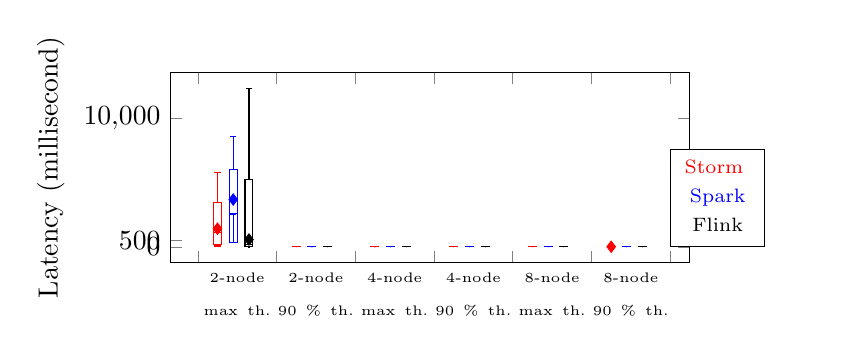
\begin{tikzpicture}

\begin{axis}[
scaled y ticks = false,
legend entries={simulation,
                measurement,
                sample 1}, 
                legend style={at={(axis cs:6.0,0.84)},anchor=south west},
boxplot/draw direction=y,
ylabel={Latency (millisecond)},
height=4cm,
boxplot={
    %
    % Idea: 
    %  place the 
    %  group 1 at 0.3333 and 0.6666
    %  group 2 at 1.3333 and 1.6666
    %  group 3 at 2.3333 and 2.6666
    %  ...
    % in a formular:
    draw position={1/4 + floor(\plotnumofactualtype/3) + 1/5*mod(\plotnumofactualtype,3)},
    %
    % that means the box extend must be at most 0.33333 :
    box extend=0.1,
},
% ... it also means that 1 unit in x controls the width:
x=1cm,
% ... and it means that we should describe intervals:
xtick={0,1,2,...,10},
ytick={0, 500,10000},
x tick label as interval,
xticklabels={%
    {\tiny 2-node \\ max th.},%
    {\tiny 2-node \\ 90 \% th.},%
    {\tiny 4-node \\ max th.},%
    {\tiny 4-node \\ 90 \% th.},%
    {\tiny 8-node \\ max th.},%
    {\tiny 8-node \\ 90 \% th.},%
},
    x tick label style={
        text width=4.5cm,
        align=center
    },
]
\addlegendimage{line legend,green}
\addlegendentry{ \textcolor{red}{\scriptsize{Storm}   }  }
\addlegendimage{line legend,blue}
\addlegendentry{\textcolor{blue}{\scriptsize{Spark}}}
\addlegendimage{line legend,blue}
\addlegendentry{\textcolor{black}{\scriptsize{Flink}}}
    % 2 node 100
\addplot[color=red,
    boxplot prepared={
      average=1407,
      lower whisker=66,
      upper whisker=5758,
      lower quartile=168,
      upper quartile=3477,
      median=1100
    },
    ] coordinates {};
    
\addplot[color=blue,
    boxplot prepared={
      average=3673,
      lower whisker=2537,
      upper whisker=8596,
      lower quartile=340,
      upper quartile=5990,
      median=2578
    },
    ] coordinates {};
    
    
\addplot[color=black,
    boxplot prepared={
      average=563,
      lower whisker=4,
      upper whisker=12328,
      lower quartile=15,
      upper quartile=5233,
      median=161
    },
    ] coordinates {};
    % 2 node 90
\addplot[color=red,
    boxplot prepared={
      median=1,
      upper quartile=1.2,
      lower quartile=0.4,
      upper whisker=1.5,
      lower whisker=0.2
    },
    ] coordinates {};
    
    
\addplot[color=blue,
    boxplot prepared={
      median=1,
      upper quartile=1.2,
      lower quartile=0.4,
      upper whisker=1.5,
      lower whisker=0.2
    },
    ] coordinates {};
\addplot[color=black,
    boxplot prepared={
      median=1,
      upper quartile=1.2,
      lower quartile=0.4,
      upper whisker=1.5,
      lower whisker=0.2
    },
    ] coordinates {};
    
        % 4 node 100
    \addplot[color=red,
    boxplot prepared={
      median=1,
      upper quartile=1.2,
      lower quartile=0.4,
      upper whisker=1.5,
      lower whisker=0.2
    },
    ] coordinates {};
    
    
\addplot[color=blue,
    boxplot prepared={
      median=1,
      upper quartile=1.2,
      lower quartile=0.4,
      upper whisker=1.5,
      lower whisker=0.2
    },
    ] coordinates {};
\addplot[color=black,
    boxplot prepared={
      median=1,
      upper quartile=1.2,
      lower quartile=0.4,
      upper whisker=1.5,
      lower whisker=0.2
    },
    ] coordinates {};
    
            % 4 node 90
    \addplot[color=red,
    boxplot prepared={
      median=1,
      upper quartile=1.2,
      lower quartile=0.4,
      upper whisker=1.5,
      lower whisker=0.2
    },
    ] coordinates {};
    
    
\addplot[color=blue,
    boxplot prepared={
      median=1,
      upper quartile=1.2,
      lower quartile=0.4,
      upper whisker=1.5,
      lower whisker=0.2
    },
    ] coordinates {};
\addplot[color=black,
    boxplot prepared={
      median=1,
      upper quartile=1.2,
      lower quartile=0.4,
      upper whisker=1.5,
      lower whisker=0.2
    },
    ] coordinates {};

            
            % 8 node 100
\addplot[color=red,
    boxplot prepared={
      median=1,
      upper quartile=1.2,
      lower quartile=0.4,
      upper whisker=1.5,
      lower whisker=0.2
    },
    ] coordinates {};
    
    
\addplot[color=blue,
    boxplot prepared={
      median=1,
      upper quartile=1.2,
      lower quartile=0.4,
      upper whisker=1.5,
      lower whisker=0.2
    },
    ] coordinates {};
\addplot[color=black,
    boxplot prepared={
      median=1,
      upper quartile=1.2,
      lower quartile=0.4,
      upper whisker=1.5,
      lower whisker=0.2
    },
    ] coordinates {};

            
            
             % 8 node 90
 \addplot[color=red,
    boxplot prepared={
      median=1,
      upper quartile=1.2,
      lower quartile=0.4,
      upper whisker=1.5,
      lower whisker=0.2,
       average = 4.05
    },
    ] coordinates {};
    
    
\addplot[color=blue,
    boxplot prepared={
      median=1,
      upper quartile=1.2,
      lower quartile=0.4,
      upper whisker=1.5,
      lower whisker=0.2
    },
    ] coordinates {};
\addplot[color=black,
    boxplot prepared={
      median=1,
      upper quartile=1.2,
      lower quartile=0.4,
      upper whisker=1.5,
      lower whisker=0.2
    },
    ] coordinates {};


\end{axis}

\end{tikzpicture}
\caption{dede}
\end{figure}
